\documentclass[pdflatex,sn-mathphys-num]{sn-jnl}

\usepackage{graphicx}
\usepackage{amsmath,amssymb,amsfonts}
\usepackage{booktabs}
\usepackage{multirow}
\usepackage{tabularx}
\usepackage{threeparttable}
\usepackage{float}
\usepackage{algorithm}
\usepackage{algorithmicx}
\usepackage{algpseudocode}
\usepackage{tikz}
\usetikzlibrary{arrows.meta,positioning,fit}

\newcommand{\method}{\textsc{SemantiFusion}}
\newcommand{\stego}{I_{\mathrm{s}}}
\newcommand{\msg}{\mathbf{m}}
\newcommand{\mhat}{\widehat{\mathbf{m}}}

\raggedbottom

\begin{document}

\title[SemantiFusion]{SemantiFusion: Message-Conditioned Semantic--Diffusion Steganography for Natural Images}

\author*[1]{\fnm{Khaled} \sur{Alrawashdeh}}\email{alrawakm@mail.uc.edu}

\affil*[1]{\orgdiv{Faculty of Computer and Information Technology},
\orgname{Jordan University of Science and Technology},
\orgaddress{\city{Irbid}, \country{Jordan}}}

\abstract{Image steganography must balance payload recovery, fidelity, and resistance to detection. This paper presents \method, a reference-conditioned latent-diffusion system in which a secret bit string and global semantic tokens jointly condition the denoising network. A vision--language encoder represents the reference image, a message encoder maps the payload to continuous tokens, and cross-attention supplies both token sets throughout reverse diffusion. The output is therefore a stochastic resynthesis of a reference image rather than a sparse pixel edit. At a 256-bit payload on $256\times256$ COCO images, the reported evaluation gives 39.2~dB PSNR, 0.96 SSIM, 3.2\% bit error rate, and 0.51 AUC under a transfer-steganalysis protocol. A payload sweep from 64 to 1024 bits changes PSNR from 40.8 to 37.6~dB and bit error rate from 1.5\% to 7.8\%. Detector AUC ranges from 0.50 to 0.55. These detector results show limited transfer from the tested steganalyzers; they do not establish security against a detector trained directly on \method{} outputs. The study consequently supports a bounded claim: semantic and message conditioning can be integrated into reference-guided diffusion with useful fidelity and recovery, while adaptive steganalysis remains necessary before deployment.}

\keywords{image steganography, latent diffusion, semantic conditioning, vision--language models, steganalysis, information hiding}

\maketitle

\section{Introduction}
\label{sec:introduction}

Steganography conceals the existence of a communication channel by placing a secret message in otherwise ordinary media. Cryptography protects the content of a message, but an encrypted object can still reveal that communication is taking place. Image steganography instead asks whether a transmitted image can carry a recoverable payload without becoming distinguishable from benign imagery \cite{cox2007digital,fridrich2009steganography}.

The usual formulation modifies a cover image. Spatial methods alter pixel values, transform-domain methods alter coefficients, and content-adaptive methods assign lower modification costs to regions in which changes are difficult to model. Rich residual models and ensemble classifiers were developed precisely to identify the small statistical shifts left by these operations \cite{fridrich2012rich,kodovsky2012ensemble}. S-UNIWARD illustrates the strength of content-adaptive distortion design, but it also illustrates the prevailing assumption: a payload is represented by controlled changes to a fixed carrier \cite{holub2014universal}.

Learned systems replace hand-designed costs with jointly trained encoders and decoders. Adversarial training, HiDDeN, SteganoGAN, and StegaStamp showed that message recovery, image fidelity, and robustness can be optimized together \cite{hayes2017generating,zhu2018hidden,zhang2019steganogan,tancik2020stegastamp}. The resulting images can be visually convincing, yet a target-aware detector may still learn artifacts specific to the encoder. XuNet and SRNet demonstrate why a visual inspection or a single generic detector is not an adequate security test \cite{xu2016structural,boroumand2019deep}.

Diffusion models offer a different design space. They generate images through a sequence of denoising operations and accept conditioning information at several stages of that sequence \cite{ho2020denoising,song2021ddim,rombach2022highresolution}. Recent hiding systems use diffusion noise, intermediate states, or model parameters as information-bearing domains \cite{yu2023cross,peng2024ldstega,kim2025diffusionstego,chen2025hiding}. This development does not remove the steganalysis problem. In particular, a message-dependent change to the diffusion noise distribution can itself become a detectable signal \cite{zhu2026rethinking}.

This paper studies \method, a reference-guided construction that combines global semantic conditioning with a binary message representation. The reference image is encoded into a latent state and semantic tokens. Message tokens are supplied to the denoising U-Net together with the semantic tokens, and a transformer decoder estimates the payload from the resulting image. Because the system begins with a reference image and reports paired PSNR and SSIM, it is more accurately described as stochastic reference-conditioned resynthesis than as coverless generation. That distinction is important: the reported fidelity metrics describe similarity to the reference, while the security experiment asks whether outputs can be distinguished from natural images.

The contributions are:

\begin{itemize}
\item a reference- and message-conditioned formulation that states explicitly where the reference image, random seed, semantic representation, and payload enter the diffusion process;
\item a fusion design that supplies semantic and message tokens to cross-attention throughout denoising and uses a separate transformer decoder for bit recovery;
\item an empirical payload analysis at 64, 256, 512, and 1024 bits per $256\times256$ image, reporting paired fidelity, recovery, and transfer-detection measurements; and
\item a security interpretation that separates observed transfer-detector performance from the stronger, unevaluated case of adaptive steganalysis.
\end{itemize}

The last point is deliberate. Stochastic sampling can diversify outputs, but stochasticity is not a security proof and does not make gradients or adaptive classification irrelevant \cite{athalye2018obfuscated}. The experimental claims in this paper are therefore limited to the stated protocol.

\section{Related Work}
\label{sec:related}

\subsection{Classical and content-adaptive steganography}

Classical image steganography modifies spatial samples or transform coefficients while controlling the resulting distortion \cite{cox2007digital,fridrich2009steganography}. Modern content-adaptive schemes use an image-dependent cost so that changes concentrate in textured or otherwise difficult-to-predict regions. S-UNIWARD defines a universal wavelet-domain distortion applicable across embedding domains \cite{holub2014universal}. These methods are evaluated against steganalyzers built from high-dimensional residual features and scalable ensemble classifiers \cite{fridrich2012rich,kodovsky2012ensemble}.

The security of an embedding algorithm depends on the cover source, payload, and warden. A result obtained with one image source or one detector cannot be treated as a detector-independent guarantee. This source dependence also applies to learned and generative systems.

\subsection{Learned hiding and learned steganalysis}

Hayes and Danezis framed hiding as an adversarial game involving an encoder, a decoder, and a steganalyzer \cite{hayes2017generating}. HiDDeN later combined message encoding with differentiable distortion layers, enabling joint optimization for recovery after common image operations \cite{zhu2018hidden}. SteganoGAN used adversarial training for high-capacity binary hiding \cite{zhang2019steganogan}, while StegaStamp emphasized physical-image channels such as printing and recapture \cite{tancik2020stegastamp}.

Learned steganalysis advanced in parallel. XuNet uses constrained early filtering and a purpose-built convolutional architecture \cite{xu2016structural}. SRNet learns residual representations directly and remains a standard target-aware baseline \cite{boroumand2019deep}. These detectors motivate a strict distinction between \emph{transfer evaluation}, in which a detector is not trained on outputs from the proposed method, and \emph{adaptive evaluation}, in which it is.

\subsection{Diffusion-based information hiding}

Diffusion models learn a reverse process that maps noise to data \cite{ho2020denoising}. DDIM provides a non-Markovian formulation that permits faster deterministic or partially stochastic sampling \cite{song2021ddim}, and latent diffusion moves the process to a compressed representation to reduce computational cost \cite{rombach2022highresolution}.

Several hiding schemes now use this machinery. CRoSS uses pretrained diffusion components for controllable image hiding without additional training \cite{yu2023cross}. LDStega encodes messages through a latent-diffusion construction designed for practical recovery \cite{peng2024ldstega}. Diffusion-Stego projects binary messages into the initial noise of a pretrained model \cite{kim2025diffusionstego}. Other work edits learned score functions so that a diffusion model stores and reconstructs secret images \cite{chen2025hiding}. These methods differ in the object being hidden, the carrier, the location of the information-bearing representation, and the receiver's required secret.

Recent steganalysis of diffusion-based generative hiding is especially relevant. Zhu et al. recover diffusion noise and classify statistical departures in that space, showing that weak performance by conventional image-domain detectors need not imply security against a method-specific warden \cite{zhu2026rethinking}. Accordingly, the present work does not treat chance-level transfer AUC as evidence of cryptographic indistinguishability.

\subsection{Semantic conditioning}

Vision--language models provide global representations of image content. CLIP learns aligned image and text embeddings from large-scale image--text pairs \cite{radford2021learning}. BLIP and BLIP-2 extend this line with bootstrapped captioning and lightweight connections between frozen image encoders and language models \cite{li2022blip,li2023blip2}. In \method, such a representation constrains reference semantics during resynthesis. It is not used to identify a fixed set of pixels in which to place the message.

Table~\ref{tab:positioning} positions the method against representative, verifiable systems. The categories are descriptive rather than rankings because the studies use different datasets, payload definitions, channels, and threat models.

\begin{table}[t]
\centering
\caption{Positioning of representative image-hiding systems. ``Adaptive detector'' indicates that security evaluation includes a detector trained on outputs from the evaluated method.}
\label{tab:positioning}
\small
\begin{tabularx}{\columnwidth}{p{2.2cm}p{2.7cm}X}
\toprule
\textbf{Method} & \textbf{Mechanism} & \textbf{Evaluation relevant here} \\
\midrule
S-UNIWARD \cite{holub2014universal} & Content-adaptive cover modification & Classical residual-feature steganalysis \\
HiDDeN; SteganoGAN \cite{zhu2018hidden,zhang2019steganogan} & Learned cover modification and neural recovery & Learned steganalyzers included in the source studies \\
CRoSS; LDStega; Diffusion-Stego \cite{yu2023cross,peng2024ldstega,kim2025diffusionstego} & Diffusion translation or latent/noise encoding & Diffusion-based hiding under method-specific protocols \\
SemantiFusion & Reference-conditioned semantic and message denoising & Transfer detectors reported; adaptive detector not reported \\
\bottomrule
\end{tabularx}
\end{table}

\section{Problem Formulation and Threat Model}
\label{sec:formulation}

Let $I\in[0,1]^{H\times W\times3}$ be a reference image, let $\msg\in\{0,1\}^{k}$ be a uniformly sampled message, and let $r$ denote the randomness used by the sampler. The sender produces
\begin{equation}
\stego = G_{\theta}(I,\msg,r),
\label{eq:generator}
\end{equation}
and the receiver estimates
\begin{equation}
\mhat = D_{\phi}(\stego).
\label{eq:decoder}
\end{equation}
Unlike a sparse embedding map, $G_{\theta}$ performs a reference-conditioned latent denoising process. The reference is nevertheless part of the construction; Equation~\eqref{eq:generator} must not be read as unconditional or strictly coverless generation.

Three objectives are measured. Recoverability is summarized by bit error rate,
\begin{equation}
\mathrm{BER}(\msg,\mhat)=\frac{1}{k}\sum_{j=1}^{k}\mathbb{1}[m_j\neq\widehat{m}_j].
\label{eq:ber}
\end{equation}
Reference fidelity is measured by PSNR and SSIM between $I$ and $\stego$. Detector performance is summarized by the area under the receiver operating characteristic curve (AUC). An AUC near 0.5 means that the evaluated detector does not rank the two classes reliably; it does not imply equality of the underlying distributions.

For a detector $A$ and matched natural and stego sources $P_{\mathrm{c}}$ and $P_{\mathrm{s}}$, a useful operational quantity is
\begin{equation}
\mathrm{Adv}_{A}=\left|\Pr_{X\sim P_{\mathrm{s}}}[A(X)=1]-
\Pr_{X\sim P_{\mathrm{c}}}[A(X)=1]\right|.
\label{eq:advantage}
\end{equation}
The empirical study estimates performance only for the tested detectors and data construction. It does not bound Equation~\eqref{eq:advantage} over all efficient distinguishers.

\subsection{Evaluated and unevaluated wardens}

The reported experiment corresponds to a passive transfer warden: the warden observes images and applies established image-domain steganalyzers, but those detectors are not trained on \method{} outputs. This setting tests whether artifacts learned from other hiding schemes transfer to the proposed generator.

The stronger adaptive setting is not evaluated. An adaptive warden would know the algorithm, collect labeled outputs from the deployed checkpoint, tune preprocessing to the generator, and train a target-specific image- or noise-domain detector. The warden might also know the vision--language encoder and diffusion backbone. The absence of this experiment is a material limitation, particularly in view of recent noise-space steganalysis \cite{zhu2026rethinking}.

The study also does not evaluate an active warden who recompresses, resizes, crops, filters, or deliberately perturbs transmitted images. Consequently, the reported clean-image BER is not a robustness result. Key establishment, decoder distribution, checkpoint compromise, chosen-message attacks, and repeated use of the same semantic reference are outside the measured scope.

\section{SemantiFusion Framework}
\label{sec:method}

\method{} has four components: a frozen vision--language encoder, a message encoder, a latent denoising network with joint cross-attention, and a transformer message decoder. Figure~\ref{fig:pipeline} shows the data flow.

\begin{figure}[t]
\centering
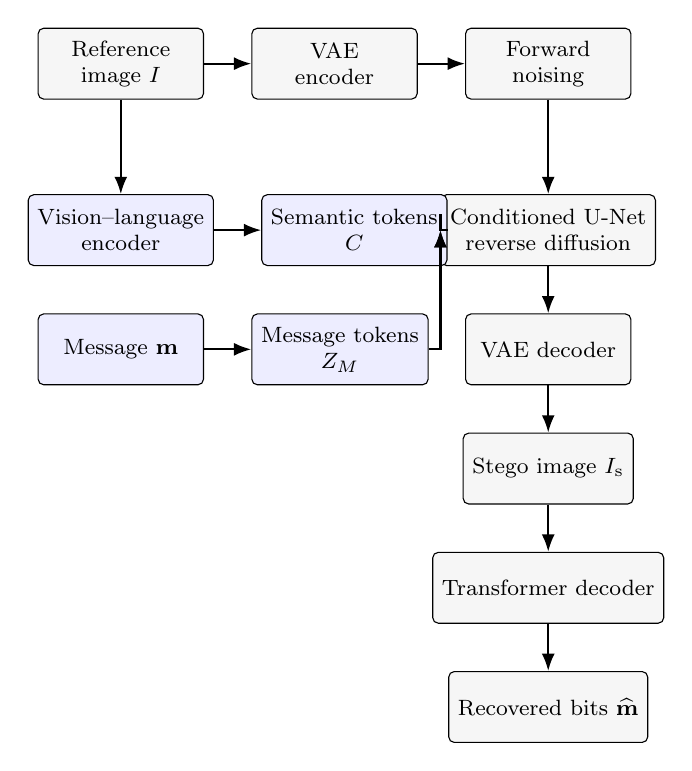
\begin{tikzpicture}[
node distance=6mm and 6mm,
box/.style={draw, rounded corners=2pt, align=center, minimum height=9mm, minimum width=21mm, font=\footnotesize, fill=gray!7},
cond/.style={draw, rounded corners=2pt, align=center, minimum height=9mm, minimum width=21mm, font=\footnotesize, fill=blue!7},
arrow/.style={-{Latex[length=2.2mm]}, thick}
]
\node[box] (ref) {Reference\\image $I$};
\node[box, right=of ref] (vaeenc) {VAE\\encoder};
\node[box, right=of vaeenc] (noise) {Forward\\noising};
\node[box, below=12mm of noise] (unet) {Conditioned U-Net\\reverse diffusion};
\node[box, below=of unet] (vaedec) {VAE decoder};
\node[box, below=of vaedec] (stego) {Stego image $\stego$};

\node[cond, below=12mm of ref] (vl) {Vision--language\\encoder};
\node[cond, right=of vl] (sem) {Semantic tokens\\$C$};
\node[cond, below=of vl] (msg) {Message $\msg$};
\node[cond, right=of msg] (mtok) {Message tokens\\$Z_M$};
\node[box, below=of stego] (decoder) {Transformer decoder};
\node[box, below=of decoder] (mhat) {Recovered bits $\mhat$};

\draw[arrow] (ref) -- (vaeenc);
\draw[arrow] (vaeenc) -- (noise);
\draw[arrow] (noise) -- (unet);
\draw[arrow] (unet) -- (vaedec);
\draw[arrow] (vaedec) -- (stego);
\draw[arrow] (ref) -- (vl);
\draw[arrow] (vl) -- (sem);
\draw[arrow] (sem) -| (unet.west);
\draw[arrow] (msg) -- (mtok);
\draw[arrow] (mtok) -| (unet.west);
\draw[arrow] (stego) -- (decoder);
\draw[arrow] (decoder) -- (mhat);
\end{tikzpicture}
\caption{\method{} pipeline. The reference image supplies a latent starting point and global semantic tokens. Message tokens and semantic tokens condition reverse diffusion through cross-attention. A separate decoder estimates the payload from the resulting image.}
\label{fig:pipeline}
\end{figure}

\subsection{Semantic representation}

A frozen vision--language image encoder maps the reference image to a sequence of semantic tokens,
\begin{equation}
C=f_{\mathrm{VL}}(I)=\{c_1,\ldots,c_N\}, \qquad c_i\in\mathbb{R}^{d}.
\label{eq:semantic}
\end{equation}
The role of $C$ is global conditioning. It represents the content of the reference without defining an embedding mask or a list of modified locations. CLIP- and BLIP-family encoders are suitable for this role because their features capture high-level visual content \cite{radford2021learning,li2022blip,li2023blip2}. The experimental archive identifies the use of a frozen vision--language encoder but does not retain an exact checkpoint identifier; this missing identifier is listed as a reproducibility limitation in Section~\ref{sec:limitations}.

\subsection{Message representation}

The message encoder first maps each bit to a trainable token and then transforms the token sequence with a multilayer perceptron:
\begin{equation}
Z_M=g_{\mathrm{msg}}(\mathrm{Embed}(\msg)), \qquad Z_M\in\mathbb{R}^{k\times d_m}.
\label{eq:message}
\end{equation}
Continuous message tokens are compatible with attention layers and avoid assigning a fixed bit to a fixed output pixel. This architectural property alone does not imply that the payload is statistically hidden; a target-aware detector may still identify population-level artifacts.

\subsection{Reference-conditioned latent diffusion}

Let $z_0=E_{\mathrm{VAE}}(I)$ be the latent representation of the reference. The forward process is
\begin{equation}
q(z_t\mid z_{t-1})=
\mathcal{N}\!\left(z_t;\sqrt{1-\beta_t}\,z_{t-1},\beta_t\mathbf{I}\right),
\label{eq:forward}
\end{equation}
where $\{\beta_t\}_{t=1}^{T}$ is the noise schedule. Equivalently,
\begin{equation}
z_t=\sqrt{\bar{\alpha}_t}z_0+\sqrt{1-\bar{\alpha}_t}\,\epsilon,
\qquad \epsilon\sim\mathcal{N}(0,\mathbf{I}).
\label{eq:closedforward}
\end{equation}
The denoising network estimates noise while conditioned on the semantic and message tokens:
\begin{equation}
\epsilon_{\theta}=\epsilon_{\theta}(z_t,t,C,Z_M).
\label{eq:denoiser}
\end{equation}
Latent features supply the queries in cross-attention; the concatenated semantic and message tokens supply keys and values. Conditioning is applied across the selected U-Net attention blocks rather than at a single output layer. After the final denoising step, the VAE decoder produces $\stego$.

The random variable $r$ in Equation~\eqref{eq:generator} includes the sampled noise and any stochastic sampling choices. Different values of $r$ can therefore produce different images for the same $(I,\msg)$ pair. DDIM sampling reduces inference cost relative to the full training schedule \cite{song2021ddim}.

\subsection{Message recovery}

The receiver converts $\stego$ to patch embeddings and passes them through a transformer decoder. A linear head yields one logit per message bit. Thresholding the sigmoid outputs gives $\mhat$. The decoder is trained jointly with message conditioning so that information distributed through the generated image remains recoverable.

The retained method description supports the standard diffusion noise-prediction term and a bit-reconstruction term. It also states that the system preserves the reference and its semantics, but the archived project does not preserve the numerical weights used to combine these objectives. We therefore write the training objective without assigning unrecorded constants:
\begin{equation}
\mathcal{L}=
\mathcal{L}_{\mathrm{diff}}
+\lambda_{\mathrm{bit}}\mathcal{L}_{\mathrm{bit}}
+\lambda_{\mathrm{ref}}\mathcal{L}_{\mathrm{ref}}
+\lambda_{\mathrm{sem}}\mathcal{L}_{\mathrm{sem}},
\label{eq:objective}
\end{equation}
where $\mathcal{L}_{\mathrm{diff}}$ is the denoising loss, $\mathcal{L}_{\mathrm{bit}}$ is binary cross-entropy on message bits, $\mathcal{L}_{\mathrm{ref}}$ penalizes departure from the reference, and $\mathcal{L}_{\mathrm{sem}}$ penalizes departure in the frozen semantic representation. Exact loss weights must be restored from the training configuration before an independent reproduction is claimed.

\subsection{Learning objectives in detail}

The diffusion term follows the noise-prediction objective used in denoising diffusion models:
\begin{equation}
\mathcal{L}_{\mathrm{diff}}
=\mathbb{E}_{z_0,t,\epsilon,\msg}
\left[
\left\|\epsilon-
\epsilon_{\theta}(z_t,t,C,Z_M)\right\|_2^2
\right].
\label{eq:diffusionloss}
\end{equation}
The expectation includes independently sampled messages so that the denoiser cannot associate a fixed payload with a particular training image. This term preserves the ordinary denoising task while allowing the conditional pathway to influence the reconstructed latent.

For a $k$-bit payload, the message-recovery term is
\begin{equation}
\mathcal{L}_{\mathrm{bit}}
=-\frac{1}{k}\sum_{j=1}^{k}
\left[m_j\log p_j+(1-m_j)\log(1-p_j)\right],
\label{eq:bitloss}
\end{equation}
where $p_j$ is the decoder probability for bit $j$. Equation~\eqref{eq:bitloss} is differentiable and directly related to BER, although minimizing cross-entropy does not guarantee a particular BER after thresholding.

Reference preservation and semantic preservation act at different scales. A reference loss may be expressed as a pixel or perceptual distance,
\begin{equation}
\mathcal{L}_{\mathrm{ref}}=d_{\mathrm{ref}}(I,\stego),
\label{eq:refloss}
\end{equation}
while semantic consistency can be expressed through normalized frozen representations,
\begin{equation}
\mathcal{L}_{\mathrm{sem}}=
1-\frac{f_{\mathrm{VL}}(I)^{\mathsf{T}}f_{\mathrm{VL}}(\stego)}
{\|f_{\mathrm{VL}}(I)\|_2\,\|f_{\mathrm{VL}}(\stego)\|_2}.
\label{eq:semloss}
\end{equation}
The first discourages visible departure from the paired reference. The second discourages a change in the representation used by the semantic encoder. Neither term establishes human semantic equivalence, and a low value of Equation~\eqref{eq:semloss} may reflect invariances or blind spots of the selected encoder.

The four terms in Equation~\eqref{eq:objective} compete. Increasing $\lambda_{\mathrm{bit}}$ can lower BER while making message-dependent structure easier to detect. Increasing $\lambda_{\mathrm{ref}}$ can improve paired PSNR while reducing the degrees of freedom available for the message. Increasing $\lambda_{\mathrm{sem}}$ can preserve the chosen representation while leaving low-level artifacts unchanged. For this reason, loss weights are experimental parameters rather than incidental implementation details.

\subsection{Conditioning across the denoising trajectory}

A single late-stage message injection would give the payload only a narrow route to the output. In \method, message and semantic tokens are available at multiple attention blocks and denoising steps. For an attention block with latent query matrix $Q_t$ and conditioning tokens $K_c,V_c$, the conditional update has the form
\begin{equation}
\mathrm{Attn}(Q_t,K_c,V_c)
=\mathrm{softmax}\!\left(\frac{Q_tK_c^{\mathsf{T}}}{\sqrt{d}}\right)V_c,
\quad [K_c;V_c]=h([C;Z_M]).
\label{eq:crossattention}
\end{equation}
This construction does not assign bit $m_j$ to a spatial coordinate. It permits the learned representation of the full message to influence many latent features. The resulting dependence is distributed, but it remains a learnable dependence: a detector trained on enough labeled outputs may identify regularities created by $h$, the U-Net, or the decoder loss.

Semantic and message conditioning also have different functions. Semantic tokens are obtained from the reference and are unchanged when only the payload changes. Message tokens change with each payload. An ablation that removes $C$ tests reference-semantic control; an ablation that removes $Z_M$ tests whether recovery is above chance; an ablation that restricts message injection to late steps tests whether trajectory-wide conditioning contributes beyond a conventional output perturbation. The supplied archive does not contain these ablation results, so they are stated as required tests rather than reported findings.

\subsection{Stochastic multiplicity and repeated-reference use}

For a fixed reference and message, the conditional distribution is
\begin{equation}
P_{I,\msg}(A)=\Pr_{r}\left[G_{\theta}(I,\msg,r)\in A\right]
\label{eq:conditionaldistribution}
\end{equation}
for measurable image sets $A$. Nonzero conditional variance means that repeated generation need not reproduce the same stego image. This property removes exact output determinism, but it creates an additional evaluation axis: variation across seeds must be measured rather than represented by a single sample.

Repeated use of one reference is particularly important. If many outputs are generated from the same $I$, an adversary can compare them to estimate the reconstruction distribution and search for message-dependent components. A realistic evaluation should therefore separate two cases: one stego output per reference and repeated outputs per reference. The latter gives the warden more information and may reveal artifacts hidden by an image-level random split.

Table~\ref{tab:components} separates the intended role of each component from the evidence needed to validate that role.

\begin{table}[t]
\centering
\caption{Component roles and the measurements needed to validate them.}
\label{tab:components}
\footnotesize
\begin{tabularx}{\columnwidth}{p{2.2cm}p{2.5cm}X}
\toprule
\textbf{Component} & \textbf{Intended role} & \textbf{Direct validation} \\
\midrule
Vision--language encoder & Preserve reference-level content & Encoder ablation and human/content-label checks \\
Message encoder & Provide continuous payload tokens & Bit-wise accuracy and payload permutation control \\
Cross-attention & Distribute conditioning across latent features & Injection-depth and timestep ablations \\
Latent diffusion & Produce stochastic reference resynthesis & Seed-wise fidelity and distributional analysis \\
Transformer decoder & Recover the complete bit string & BER, calibration, and per-bit error profile \\
\bottomrule
\end{tabularx}
\end{table}

\begin{algorithm}[t]
\caption{Reference-conditioned message generation and recovery}
\label{alg:semantifusion}
\begin{algorithmic}[1]
\Require Reference image $I$, message $\msg$, random seed $r$
\State $C\gets f_{\mathrm{VL}}(I)$
\State $Z_M\gets g_{\mathrm{msg}}(\mathrm{Embed}(\msg))$
\State $z_0\gets E_{\mathrm{VAE}}(I)$
\State Sample $z_t$ from $z_0$ using seed $r$
\For{$s=t,t-1,\ldots,1$}
  \State $\widehat{\epsilon}\gets\epsilon_{\theta}(z_s,s,C,Z_M)$
  \State $z_{s-1}\gets\mathrm{Step}(z_s,\widehat{\epsilon},s,r)$
\EndFor
\State $\stego\gets D_{\mathrm{VAE}}(z_0)$
\State $\mhat\gets D_{\phi}(\stego)$
\State \Return $\stego,\mhat$
\end{algorithmic}
\end{algorithm}

\section{Experimental Design}
\label{sec:experiment}

\subsection{Datasets and preprocessing}

MS-COCO contains varied natural scenes and object combinations \cite{lin2014microsoft}. The reported primary evaluation uses the 5,000 images in the 2017 validation split, resized to $256\times256$ pixels with bicubic interpolation. The model description states that fine-tuning used COCO training images; the validation split is reserved for the reported primary measurements.

DIV2K provides 1,000 high-resolution images developed for image-restoration evaluation \cite{agustsson2017ntire}. The reported protocol uses its 100-image validation subset, with center cropping and resizing to $256\times256$. BOSSBase v1.01 contains 10,000 grayscale photographs from multiple cameras \cite{bas2011break}. The protocol replicates the grayscale channel into RGB and resizes each image to $256\times256$.

Messages are independent, uniformly sampled binary strings. Payloads are 64, 256, 512, and 1024 bits per image. At the stated resolution these correspond to approximately 0.0010, 0.0039, 0.0078, and 0.0156 bits per pixel (bpp), respectively. This bpp definition divides message length by the number of spatial pixels, not by the number of color samples.

\subsection{Metrics}

PSNR and SSIM measure similarity between the reference image and its resynthesized output. SSIM compares luminance, contrast, and structure \cite{wang2004image}. BER is defined in Equation~\eqref{eq:ber}. AUC measures a detector's ability to rank stego images above natural images. The metrics answer different questions: a high PSNR does not imply a low BER, and neither metric establishes resistance to steganalysis.

\subsection{Implementation retained in the experiment record}

Table~\ref{tab:implementation} lists the implementation information available in the source project. Values absent from the project are not reconstructed from defaults because such substitutions would change the experimental specification.

\begin{table}[t]
\centering
\caption{Implementation details retained in the source project.}
\label{tab:implementation}
\begin{tabularx}{\columnwidth}{p{3.1cm}X}
\toprule
\textbf{Item} & \textbf{Recorded value} \\
\midrule
Operating system & Ubuntu 22.04 LTS \\
Framework & Python 3.10; PyTorch 2.0 \\
GPU & NVIDIA RTX A6000, 48 GB \\
CPU and memory & 24-core Intel Xeon Gold-class CPU; 128 GB RAM \\
Optimizer & AdamW \\
Initial learning rate & $5\times10^{-5}$ \\
Batch size & 64 \\
Fine-tuning duration & 50 epochs \\
Diffusion schedule & 1,000 training steps; 50 DDIM inference steps \\
Stopping rule & Validation BER \\
Image resolution & $256\times256$ RGB \\
\bottomrule
\end{tabularx}
\end{table}

The project describes a pretrained latent-diffusion backbone fine-tuned with random messages and a jointly trained transformer decoder. All runs use fixed random seeds. The exact pretrained checkpoint, vision--language checkpoint, seed list, loss weights, optimizer weight decay, and train/validation manifest are not present in the archived project. These omissions do not alter the aggregate values reported below, but they prevent a bit-for-bit independent reproduction from the manuscript alone.

\subsection{Steganalysis protocol}

The retained protocol forms a balanced test collection of 5,000 stego images and 5,000 natural images and reports results for SRM/SRNet-family image-domain analysis. The key constraint is that no detector was trained directly on \method{} outputs. The result is therefore a transfer test, not a targeted adaptive test. This wording resolves a contradiction in the earlier draft, which simultaneously stated that detectors were trained from scratch and that they were not trained on \method{} images.

Baseline rows for HiDDeN and SteganoGAN are retained because both methods and their source publications are verifiable. The earlier ``semantic baseline'' row is removed: its citation could not be resolved to a published source, so retaining it would make the comparison unverifiable. The baseline values below are the values reported in the project at a common 256-bit payload and image resolution; they should not be read as values copied from the original baseline papers.

\section{Results}
\label{sec:results}

\subsection{Primary 256-bit comparison}

Table~\ref{tab:primary} reports the primary comparison. At 256 bits, \method{} records 39.2~dB PSNR, 0.96 SSIM, 3.2\% BER, and 0.51 transfer-detector AUC. Relative to the two retained local baselines, the reported output has higher paired fidelity and lower clean-image BER. AUC is also closer to 0.5, which shows that the tested detector transfers poorly to this output distribution.

\begin{table}[t]
\centering
\caption{Reported COCO results at a 256-bit payload and $256\times256$ resolution.}
\label{tab:primary}
\begin{tabular}{lcccc}
\toprule
\textbf{Method} & \textbf{PSNR} & \textbf{SSIM} & \textbf{BER} & \textbf{AUC} \\
& \textbf{(dB)} & & \textbf{(\%)} & \\
\midrule
HiDDeN \cite{zhu2018hidden} & 36.9 & 0.94 & 6.4 & 0.61 \\
SteganoGAN \cite{zhang2019steganogan} & 37.4 & 0.95 & 5.7 & 0.58 \\
\method{} & \textbf{39.2} & \textbf{0.96} & \textbf{3.2} & \textbf{0.51} \\
\bottomrule
\end{tabular}
\end{table}

These numbers are descriptive aggregates. Run-level predictions and repeated-training records are not present in the source package, so confidence intervals, variance across seeds, and paired significance tests cannot be reconstructed. The table should therefore not be used to claim statistically established superiority.

\subsection{Qualitative COCO examples}

Figure~\ref{fig:qualitative-coco} restores three original--stego comparisons retained in the supplied experiment archive. The artifact identifies COCO val2017 images 000000000139, 000000000632, and 000000000724. No large structural change is visible in these three pairs at the printed scale.

The archive contains the composite figure but not the six image files, payloads, generation seeds, or generating checkpoint. The figure is used only as a qualitative record. It does not support a per-image metric or a perceptual-study claim. The companion package records its SHA-256 digest and archive path.

\begin{figure}[H]
\centering
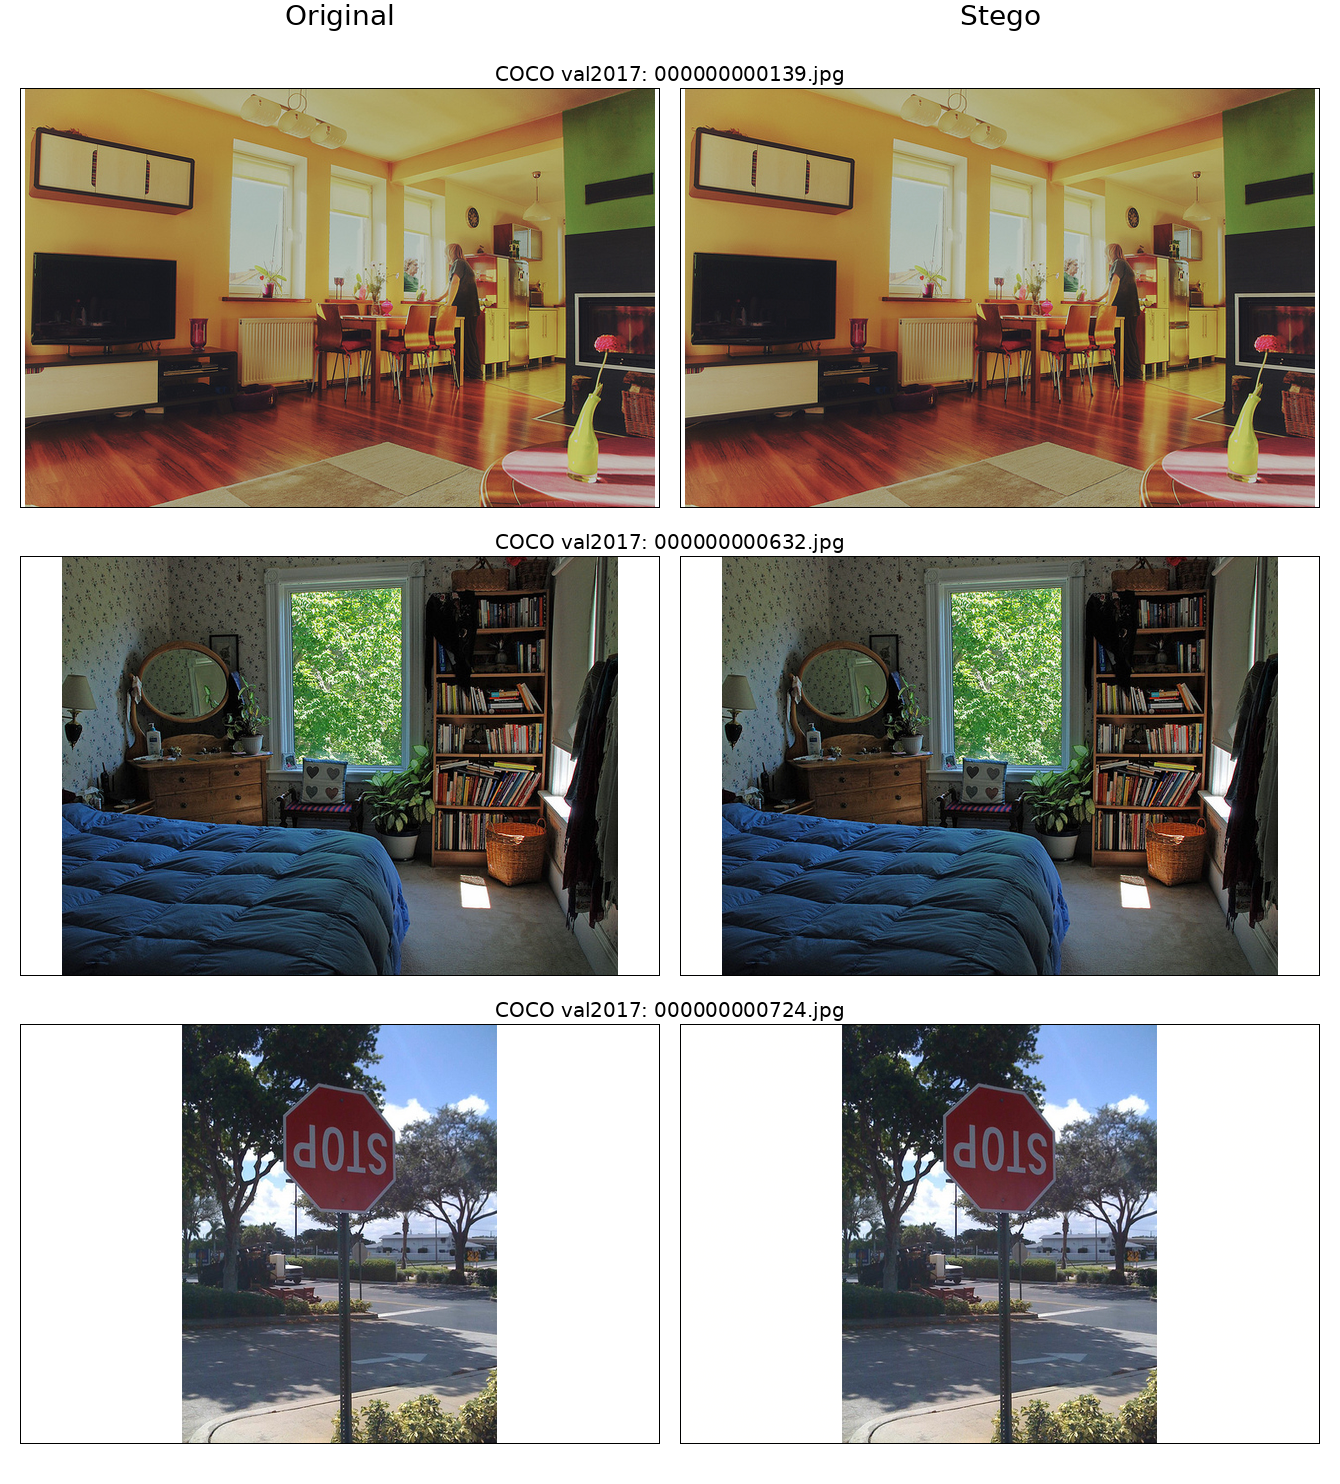
\includegraphics[width=0.86\textwidth]{figures/qualitative_coco_pairs.png}
\caption{Three COCO val2017 pairs retained in the archive. Each row shows the reference image on the left and the recorded stego image on the right. The identifiers are part of the source figure. Raw images and generation logs were unavailable, so no per-image metric was calculated from this composite.}
\label{fig:qualitative-coco}
\end{figure}

\subsection{Payload scaling}

Table~\ref{tab:payload} exposes the main trade-off. Increasing payload from 64 to 1024 bits reduces PSNR by 3.2~dB, reduces SSIM from 0.98 to 0.94, and increases BER by 6.3 percentage points. Transfer-detector AUC rises from 0.50 to 0.55. The trend is internally consistent: more message information places greater pressure on both reference fidelity and decoding reliability, while also making the outputs easier for the tested detector to rank.

\begin{table}[t]
\centering
\caption{Reported payload scaling on COCO at $256\times256$ resolution.}
\label{tab:payload}
\begin{tabular}{rrrrr}
\toprule
\textbf{Bits} & \textbf{bpp} & \textbf{PSNR (dB)} & \textbf{BER (\%)} & \textbf{AUC} \\
\midrule
64   & 0.0010 & 40.8 & 1.5 & 0.50 \\
256  & 0.0039 & 39.2 & 3.2 & 0.51 \\
512  & 0.0078 & 38.4 & 5.1 & 0.53 \\
1024 & 0.0156 & 37.6 & 7.8 & 0.55 \\
\bottomrule
\end{tabular}
\end{table}

The original abstract described PSNR above 39~dB and AUC no greater than 0.52 across the payload range. Table~\ref{tab:payload} does not support those statements: the 512- and 1024-bit conditions have PSNR below 39~dB and AUC above 0.52. The corrected summary reports the observed ranges instead.

\subsection{Cross-dataset evidence}

The source manuscript states that DIV2K and BOSSBase follow the same qualitative pattern, with PSNR within 1~dB of the COCO result and AUC below 0.56. It does not preserve per-dataset tables, sample-level predictions, or uncertainty estimates. For that reason, these observations are not used as evidence for a quantitative cross-dataset claim. A revised experiment should report each dataset separately, preserve the detector scores, and keep preprocessing fixed or analyze it as a factor.

\section{Security Interpretation}
\label{sec:security}

\subsection{What the transfer result shows}

The transfer AUC indicates that the tested image-domain detector does not carry its decision boundary effectively to \method{} outputs. This is useful evidence about detector mismatch. The generator does not add the same type of residual produced by the baseline encoders, and its resynthesis pathway can shift the relevant artifacts away from those learned on conventional cover modifications.

The result does not show that $P_{\mathrm{s}}=P_{\mathrm{c}}$, that message presence is information-theoretically hidden, or that all efficient wardens have negligible advantage. A target-aware detector could learn generator-specific color, texture, frequency, semantic, or reconstructed-noise statistics. Diffusion-specific steganalysis makes this possibility concrete \cite{zhu2026rethinking}.

\subsection{Feature-based steganalysis}

Rich-model steganalysis represents an image through many quantized residual co-occurrences \cite{fridrich2012rich}. For conventional additive embedding, one can write a simplified residual relation as
\begin{equation}
R(\stego)=R(I)+\delta(I,\msg),
\label{eq:additiveresidual}
\end{equation}
where $R$ is a residual operator and $\delta$ is the change created by the embedding rule. A content-adaptive algorithm aims to make $\delta$ difficult to distinguish from the cover-source residuals.

Reference-conditioned diffusion does not generally satisfy the additive form in Equation~\eqref{eq:additiveresidual}. Its output contains reconstruction error, sampling variation, and message-conditioned variation. That mismatch can explain poor transfer from a detector trained on additive residuals. It does not mean the new residual distribution is natural. A warden can instead learn
\begin{equation}
R(\stego)=R(I)+\delta_{\mathrm{rec}}(I,r)
+\delta_{\mathrm{msg}}(I,\msg,r),
\label{eq:decomposedresidual}
\end{equation}
where the two terms need not be separable in practice. The security question is whether the combined distribution differs reliably from the matched benign pipeline, not whether a classical additive model fits it.

This point determines the correct negative class. Comparing resynthesized stego images with camera-native natural images can expose generic diffusion reconstruction artifacts. Comparing them with benign reference-conditioned reconstructions produced without a message isolates message conditioning more directly. Both comparisons are useful, but they answer different questions: operational detection versus mechanism attribution.

\subsection{Target-aware deep steganalysis}

An adaptive image-domain detector should be trained on outputs from the frozen \method{} checkpoint. Reference identities must be grouped so that different outputs from one reference cannot appear in both training and test sets. If the split is made at the image-file level, a detector may exploit reference content or near-duplicate structure rather than the presence of a payload.

The detector should be trained under several payload conditions. A fixed-payload detector estimates performance at one operating point; a mixed-payload detector tests whether the method remains detectable when message length varies. The natural and stego sets must share file format, quantization, resizing, and metadata processing. A simple metadata-only classifier should be reported as a leakage control before image pixels are used.

Evaluation should include ROC AUC, balanced accuracy at a validation-selected threshold, false-positive rate at a low false-negative operating point, and calibration. AUC alone can hide behavior important to a practical warden. Confidence intervals should be computed over independent reference groups, not over individual seed replicates treated as independent images.

\subsection{Noise-space and inversion-based analysis}

Diffusion-specific wardens can attempt to invert an observed image into a latent or noise representation and then test that representation for distributional shifts. Let $J$ be an approximate inversion operator. A noise-space detector evaluates
\begin{equation}
A_{z}(\stego)=a\!\left(\psi(J(\stego))\right),
\label{eq:noisedetector}
\end{equation}
where $\psi$ extracts statistics in the recovered latent or a transform domain and $a$ is a classifier. Such a detector need not recover the secret message. It only needs to separate the message-conditioned noise distribution from the benign distribution.

This attack is relevant even though \method{} begins from a reference latent rather than projecting bits directly into an unconditional initial noise vector. Conditioning can still alter denoising trajectories or reconstructed latent statistics. A useful experiment would compare four sets: natural images, benign reconstructions, message-conditioned reconstructions, and message-conditioned reconstructions with permuted decoder labels. That design separates generic reconstruction artifacts from payload-dependent artifacts.

\subsection{Black-box transfer and surrogate access}

The current AUC belongs to a black-box transfer setting: the detector has no method-specific training set. Transfer can fail because the feature distribution differs, the preprocessing differs, or the decision threshold is unsuitable. Those explanations should not be collapsed into a single claim of undetectability.

A stronger black-box warden may query the sender, collect images, and train a surrogate without knowing the checkpoint. Query access converts the problem into supervised adaptation. The number of queries then becomes part of the threat model. Reporting detection as a function of 100, 1,000, and 10,000 labeled outputs would reveal whether the apparent security is a data-scarcity effect or a persistent distributional match.

\subsection{Why stochasticity is not a guarantee}

For fixed $(I,\msg)$, changes in the sampler seed may yield multiple outputs. This multiplicity can frustrate exact template matching and makes a one-to-one pixel interpretation less useful. It does not prevent population-level classification. A detector needs only a stable difference between the natural and generated distributions; individual outputs need not be deterministic.

Similarly, long computational graphs and stochastic samplers do not by themselves block gradient-based analysis. Randomized or non-smooth operations can produce misleading gradients, but established adaptive procedures can differentiate through expectations, approximations, or surrogate pipelines \cite{athalye2018obfuscated}. Accordingly, the method makes no claim of ``gradient obfuscation'' as a security property.

\subsection{Information carried by the image}

Successful decoding requires dependence between the message and the received image. In particular, $I(\msg;\stego)$ cannot be approximately zero if $D_{\phi}$ recovers $\msg$ with error below chance. The security objective concerns a different variable: whether an observer can infer that the image was produced by the steganographic channel. Let $S\in\{0,1\}$ indicate benign or stego origin. The detection objective is to reduce information about $S$ in the observable image while retaining enough information about $\msg$ for the authorized receiver.

These requirements are not contradictory because the receiver has side information in the form of $D_{\phi}$ and its configuration. They do, however, create a security obligation: the manuscript must state what part of the receiver is secret. If the decoder weights are public, the warden can use them as a feature extractor or test candidate messages. If the decoder is secret, the system relies on a large learned object as key material and must address distribution, revocation, and compromise. The present experiment does not resolve that design choice.

\subsection{Model exposure and chosen-message testing}

Under Kerckhoffs's principle, the algorithm should remain secure when its design is public and only a compact key is secret. The retained \method{} description does not define a compact stego key separate from the trained decoder. It is therefore more accurate to describe the current system as a learned shared-decoder channel than as a complete cryptographic protocol.

A model-aware warden can also perform chosen-message tests. It can generate outputs for all-zero, all-one, balanced random, and structured payloads and compare their features. If the message encoder maps these classes to systematically different regions of token space, the difference may propagate to the output. Training uses uniformly random messages, which covers the balanced case well but does not by itself establish invariance to low-entropy or structured payloads. Encryption before hiding would make operational payloads closer to uniform, but encryption and key management are outside the present evaluation.

\subsection{Reference fidelity and distributional realism}

Paired PSNR and SSIM establish that an output remains close to its reference. They do not establish that a population of outputs follows the natural-image distribution. Conversely, an unconditional generative model may have realistic population statistics while producing no image paired closely enough with a particular reference to yield high PSNR. The two properties should not be conflated.

This distinction affects experimental design. A rigorous evaluation needs both paired fidelity metrics and unpaired distributional or detection tests. It must also ensure that natural and stego samples share acquisition, resizing, compression, color-processing, and file-format pipelines. Otherwise, the detector can learn the data pipeline rather than the message-bearing mechanism.

\section{Discussion}
\label{sec:discussion}

\subsection{Interpretation of the method}

\method{} lies between cover modification and unconditional generative steganography. It begins with a real reference image, encodes that image into a latent state, and produces a nearby resynthesis through message-conditioned denoising. Calling the method strictly coverless would obscure this dependence and would make paired PSNR difficult to interpret. ``Reference-conditioned generative steganography'' describes the construction more precisely.

The semantic encoder has a narrow role: it supplies a global constraint intended to keep the resynthesis consistent with the reference content. It does not make the payload itself semantic, and it does not prove invariance under a change of vision--language backbone. Testing several frozen encoders and reporting their checkpoint identifiers would separate a general architectural effect from a model-specific effect.

\subsection{Relationship to semantic steganography}

Semantic steganography is used for several distinct ideas in the literature: selecting perceptually tolerant regions, encoding a message in high-level content, and constraining a generator with semantic representations. \method{} belongs to the third category. It does not infer a saliency mask, and its payload remains an ordinary binary vector. The semantic representation constrains the reference-conditioned generation process; it is not itself the secret channel.

This distinction avoids an unsupported causal claim. A high cosine similarity in the frozen encoder does not show that semantics caused the reported detector AUC, and removing pixel masks does not show that fixed structure has disappeared from every learned feature space. A controlled experiment would compare identical diffusion and decoding components with and without semantic tokens while keeping the message encoder, training images, loss weights, and seeds fixed.

The choice of semantic encoder also changes the invariances being encouraged. CLIP, BLIP, and BLIP-2 are trained with different objectives and data \cite{radford2021learning,li2022blip,li2023blip2}. Agreement under one encoder may not transfer to another. Reporting multiple encoders or downstream content labels would make semantic preservation less dependent on a single representation.

\subsection{Capacity and recovery}

The payload range is modest in bpp because the images contain 65,536 spatial pixels. Even so, the sweep shows a measurable fidelity--recovery trade-off. At 1024 bits, BER is 7.8\%, which is too high for direct error-free communication. A practical system would require an error-correcting code, but redundancy would reduce net payload. Future work should report gross payload, code rate, and net decoded payload separately.

Clean-image BER is also insufficient for an operational channel. Messaging services commonly resize and recompress images; storage systems may change metadata or color profiles. JPEG quality sweeps, resizing, additive noise, cropping, filtering, and repeated save cycles should be evaluated with identical random messages and confidence intervals.

Capacity should be reported together with reliability. For a raw payload of $k$ bits and an error-correcting code of rate $\rho$, the net information is at most $\rho k$ bits before accounting for synchronization, framing, and authentication. If the channel error pattern is bursty or correlated across bit positions, the code must be selected from the observed error structure rather than from mean BER alone. Per-bit error heat maps and error correlations would therefore be more informative than a single average.

The payload sweep also suggests that one operating point should not stand for the method. The 64-bit condition has the best fidelity and recovery, while the 1024-bit condition has the highest capacity and the weakest reported values. Applications should select an operating point based on a stated maximum BER, minimum fidelity, and detector tolerance rather than maximizing only the number of bits.

\subsection{Generalization across image sources}

COCO, DIV2K, and BOSSBase differ in content, native resolution, camera pipelines, and color representation. Resizing all images to $256\times256$ creates a common model input, but it also introduces a shared interpolation signature. BOSSBase requires channel replication, which is an especially strong domain marker. A detector may learn these source differences unless train and test construction is carefully matched.

Cross-dataset evaluation should therefore distinguish two questions. In a fixed-generator test, the generator is trained on one source and evaluated on another without adaptation. In a source-matched test, both benign and stego examples come from the same held-out source and share preprocessing. The first measures generator transport; the second measures detection within a source. The ranges retained in the archive do not reveal which effects dominate.

Camera-model and content-category holdouts would add useful structure. If a detector fails only when cameras or semantic categories change, the result is a domain-transfer limitation of the detector, not necessarily a property of the hiding system. Grouped splits and per-source results are needed to make that distinction.

\subsection{Computational cost}

Fifty DDIM steps are substantially more expensive than a single feed-forward embedding pass. The archived experiment does not include wall-clock generation time, decoder latency, peak memory, or energy use. Those measurements are needed before comparing practicality with HiDDeN or SteganoGAN. They should be reported on the same hardware with warm-up runs and a fixed batch size.

Training cost and deployment cost should be separated. The sender executes the VAE encoder, repeated U-Net evaluations, and the VAE decoder. The receiver executes only the message decoder if no verification or inverse diffusion is required. This asymmetry may be acceptable for offline publication workflows but not for interactive messaging or low-power devices. Reduced-step samplers, distilled diffusion backbones, or cached reference semantics could lower sender cost, but each change may alter both BER and detectability.

\subsection{Extension to other media}

The formulation in Equation~\eqref{eq:generator} is not limited to still images. Audio diffusion could condition waveform or spectrogram generation on a binary message, while video diffusion could distribute conditioning across spatial and temporal latent variables. The security measurements would need to change with the medium. Audio wardens can exploit spectral and phase statistics; video wardens can exploit temporal inconsistency and codec behavior.

Multimodal carriers introduce an additional attribution problem. If text, image, and audio are jointly generated, detection may arise from cross-modal inconsistency even when each modality appears natural in isolation. A semantic encoder can help align content, but it can also create a recognizable dependence shared across outputs. The present image experiment establishes no result for those channels; the extension is architectural, not empirical.

\subsection{Deployment boundaries}

A complete deployment requires more than a trained generator and decoder. The sender and receiver need message framing, error detection, key or decoder provisioning, version negotiation, and a policy for model updates. A checkpoint change may break recovery even when output images remain visually similar. Version identifiers cannot simply be stored as ordinary metadata if the metadata itself reveals use of the channel.

Transport transformations must also be specified. A method evaluated only on lossless PNG images may fail when a platform converts images to JPEG, strips color profiles, or downsamples them. Operational testing should reproduce the exact service pipeline rather than applying isolated distortions in arbitrary order. The output format and quantization settings belong in the protocol.

\subsection{Responsible use}

Image hiding supports legitimate applications such as ownership metadata, provenance, and covert communication under censorship. The same capability can be used for data exfiltration or coordination that evades monitoring. The present study uses public image datasets and does not involve human participants or personal data. Any release of trained hiding and decoding checkpoints should be accompanied by clear use conditions and by detector-oriented evaluation artifacts.

\section{Limitations and Required Validation}
\label{sec:limitations}

The current evidence has five limits.

\begin{enumerate}
\item \textbf{No adaptive detector.} The AUC values come from transfer steganalysis. A detector trained directly on \method{} outputs is the most important missing experiment.
\item \textbf{No uncertainty estimates.} Only aggregate values are available. Replicate-level results are required for confidence intervals, paired comparisons, and sensitivity to random seeds.
\item \textbf{Incomplete configuration provenance.} Exact model checkpoints, loss weights, seed list, and split manifests are absent from the archived project.
\item \textbf{No active-channel evaluation.} The reported BER applies to clean outputs and does not establish robustness after compression, resizing, cropping, or filtering.
\item \textbf{Limited cross-dataset records.} DIV2K and BOSSBase are described only by ranges, so the manuscript does not make a numerical generalization claim from them.
\end{enumerate}

These limits define a concrete validation plan. The next experiment should freeze the generator, create disjoint image-level train, validation, and test splits, train SRNet and a diffusion-noise detector on generated outputs, and report ROC curves with bootstrap confidence intervals. It should repeat training across seeds and preserve the sample manifest, detector scores, checkpoints, and environment lock file. This is more informative than adding another transfer detector.

\section{Conclusion}
\label{sec:conclusion}

This paper presented \method, a reference-conditioned latent-diffusion system for binary image hiding. Global semantic features and learned message tokens condition the reverse diffusion process, and a transformer decoder recovers the payload from the resynthesized image. The recorded COCO evaluation shows useful paired fidelity and clean-image recovery: at 256 bits, PSNR is 39.2~dB, SSIM is 0.96, and BER is 3.2\%. Across 64--1024 bits, the results show the expected capacity trade-off, with PSNR decreasing and BER increasing as the payload grows.

The transfer detector produces AUC values of 0.50--0.55. This finding is evidence that the tested image-domain detector does not transfer strongly to the generated outputs. It is not evidence that an adaptive warden will fail. The appropriate next step is therefore a target-aware image- and noise-domain steganalysis study with complete run-level records. Within that boundary, the results support semantic and message conditioning as a workable diffusion-based hiding design and identify the experiments required to evaluate its security.

\begin{appendices}

\section{Reproducibility Record}
\label{app:reproducibility}

An independently auditable experiment requires a record that connects each reported number to the images, model versions, messages, and detector outputs used to compute it. Aggregate tables alone cannot reveal duplicated samples, split overlap, failed runs, or seed sensitivity. Table~\ref{tab:manifest} gives the minimum session-level manifest for a reproducibility release.

\begin{table}[!h]
\centering
\caption{Minimum fields for a generation and evaluation manifest.}
\label{tab:manifest}
\footnotesize
\begin{tabularx}{\columnwidth}{p{2.5cm}p{1.8cm}X}
\toprule
\textbf{Field} & \textbf{Type} & \textbf{Purpose} \\
\midrule
\texttt{sample\_id} & string & Immutable key shared by images and metric rows \\
\texttt{reference\_id} & string & Groups all outputs derived from one reference \\
\texttt{dataset\_split} & category & Records source, version, and train/validation/test role \\
\texttt{payload\_bits} & integer & Distinguishes the four payload conditions \\
\texttt{message\_hash} & checksum & Binds the payload without publishing its content \\
\texttt{generation\_seed} & integer & Reproduces the stochastic sampling path \\
\texttt{model\_hash} & checksum & Identifies diffusion, semantic, and decoder checkpoints \\
\texttt{preprocess\_hash} & checksum & Identifies resize, color, quantization, and output settings \\
\texttt{output\_hash} & checksum & Binds the exact evaluated image \\
\texttt{psnr}, \texttt{ssim} & numeric & Stores paired fidelity measurements \\
\texttt{bit\_errors} & integer & Preserves the numerator used for BER \\
\texttt{detector\_score} & numeric & Preserves continuous scores used for ROC analysis \\
\texttt{status} & category & Records success, failure, exclusion, and reason \\
\bottomrule
\end{tabularx}
\end{table}

The split must be assigned at the reference level before output generation. All seeds and payload variants derived from one reference inherit that split. Dataset checksums should be recorded before preprocessing, and derived images should be stored losslessly when the experiment claims a lossless channel. If an external platform is part of the channel, both the uploaded and downloaded files require hashes.

Checkpoint provenance includes the base diffusion identifier, VAE, semantic encoder, message encoder, decoder, and any fine-tuned U-Net weights. A textual model name is insufficient when repositories can update files without changing a short label. A cryptographic checksum and the source revision should both be retained.

The environment record should include the operating system image, GPU model and driver, CUDA and cuDNN versions, Python version, package lock file, and the exact command used for each stage. Deterministic flags and known nondeterministic operators should be reported separately. A fixed seed does not guarantee identical GPU execution when kernels are nondeterministic.

\clearpage
\section{Target-Aware Steganalysis Protocol}
\label{app:adaptive_protocol}

The following protocol addresses the principal limitation of the current evaluation. It is prospective: no result from this protocol is included in Tables~\ref{tab:primary} or \ref{tab:payload}.

\subsection{Generation and grouping}

Freeze the full sender and receiver before constructing the steganalysis set. Select disjoint reference-level training, validation, and test partitions. For every reference, generate a benign reconstruction without message conditioning and message-conditioned outputs for each payload. Use more than one seed per reference, but keep every derivative of a reference in the same partition.

The natural comparison set should be processed through the same resizing, color conversion, quantization, and file-writing code. Two negative classes should be retained:
\begin{enumerate}
\item natural images, for operational detection of the complete generation pipeline; and
\item benign reconstructions, for attribution of artifacts specifically to message conditioning.
\end{enumerate}
Reporting only the easier of these tasks would obscure whether the detector recognizes diffusion reconstruction or the hidden-message mechanism.

\subsection{Detector training}

Train at least one image-domain residual network and one inversion- or noise-space detector. Hyperparameters and thresholds must be selected on the validation partition only. Class balance should be explicit; if balanced mini-batches are used while deployment prevalence is low, calibrated probabilities must be assessed under the deployment prior.

Detector development should include three controls. A metadata-only classifier tests file leakage. A reference-identity classifier tests whether content groups are separable. A payload-permutation control assigns stego labels independently of true message conditioning and should return chance performance. Failure of any control invalidates the corresponding detector result.

Train separate detectors at each payload and a mixed-payload detector. The separate models estimate detectability at a defined operating point. The mixed model tests whether one warden can recognize the family without knowing the message length. Repeat detector training with independent initialization seeds and retain every score vector.

\subsection{Evaluation and uncertainty}

The untouched test partition is evaluated once after model selection. Report ROC AUC, balanced accuracy, sensitivity, specificity, and the false-positive rate at a prespecified true-positive rate. Confidence intervals should resample reference groups so that multiple seeds from one reference remain together. A paired bootstrap can compare detectors on the same test references.

For $B$ bootstrap samples with metric estimates $\widehat{\theta}^{(1)},\ldots,\widehat{\theta}^{(B)}$, a percentile interval is
\begin{equation}
\left[
Q_{\alpha/2}(\widehat{\theta}^{(1:B)}),
Q_{1-\alpha/2}(\widehat{\theta}^{(1:B)})
\right],
\label{eq:bootstrap}
\end{equation}
where $Q$ is the empirical quantile. The resampling unit, number of bootstrap draws, and random seed must be stated. Image-level resampling would give intervals that are too narrow when several outputs share a reference.

\section{Active-Channel and Ablation Reporting}
\label{app:reporting}
\setcounter{table}{0}

An active-channel matrix should apply the same transformations to all methods and should report net payload after error correction. At minimum, the matrix should include JPEG quality, scale factor, crop fraction, additive-noise level, and repeated save cycles. Severity values and operation order must be fixed before evaluation.

\begin{table}[!h]
\centering
\caption{Minimum active-channel result matrix for each payload. Entries should report BER with a reference-group confidence interval.}
\label{tab:channelmatrix}
\footnotesize
\begin{tabularx}{\columnwidth}{p{2.3cm}p{2.2cm}X}
\toprule
\textbf{Channel} & \textbf{Levels} & \textbf{Required accompanying record} \\
\midrule
No transform & Native PNG & File hash and quantization settings \\
JPEG & Q=90, 70, 50 & Library, chroma subsampling, and encoder options \\
Resize & 0.75, 0.50 & Interpolation kernel and restoration size \\
Crop & 5\%, 10\%, 20\% & Crop policy, position, and padding rule \\
Gaussian noise & Fixed $\sigma$ grid & Value range and clipping behavior \\
Repeated save & 2, 5 cycles & Full order of decoding and encoding operations \\
\bottomrule
\end{tabularx}
\end{table}

Ablations should use the same references, messages, and seeds as the full model. The minimum set removes semantic tokens, removes message conditioning, restricts message injection to late denoising steps, replaces the transformer decoder with a capacity-matched convolutional decoder, and disables reference or semantic losses one at a time. Each ablation should report PSNR, SSIM, BER, generation time, transfer AUC, and adaptive AUC. A component is supported only when its removal changes the metric associated with its stated role.

The final release should include machine-readable metric tables rather than values copied only into LaTeX. A plotting script should read those tables directly, and every table in the manuscript should be reproducible from a single documented command. This practice prevents transcription errors and makes later detector re-evaluation possible without regenerating images.

\end{appendices}

\backmatter

\bmhead{Acknowledgements}
The author thanks the maintainers of the public datasets and open research implementations used in this study.

\section*{Declarations}

\noindent\textbf{Funding.}
The author received no external funding for this work.\par

\noindent\textbf{Competing interests.}
The author declares no competing interests.\par

\noindent\textbf{Ethics approval.}
This study used public image datasets and did not involve human participants, animals, or personally identifiable information.\par

\noindent\textbf{Data availability.}
MS-COCO, DIV2K, and BOSSBase are available from their respective maintainers. The companion artifact records the identifiers shown in the retained qualitative figure and provides schemas for image-level manifests. The source archive does not contain the run-level predictions, trained checkpoints, raw original--stego pairs, or split manifests required to reproduce the reported tables or regenerate the qualitative outputs exactly.\par

\noindent\textbf{Code availability.}
The companion artifact is prepared for release at \url{https://github.com/alrawakm/SemantiFusion-Reproducibility}. It contains the aggregate tables in machine-readable form, provenance checks, paired-image metric code, manifest validation, qualitative-figure utilities, and a target-aware evaluation protocol. It does not contain the original training program or trained generator and decoder checkpoints, which were not retained in the supplied project; consequently, the published outputs cannot yet be regenerated from weights. This limitation is stated in the repository and in Section~\ref{sec:limitations}.

\bibliography{references}

\end{document}
